% !TeX program = xelatex
\documentclass[UTF8,zihao=-4]{ctexart}

% -------------------- 页面与基础设置 --------------------
\usepackage[a4paper,margin=2.5cm]{geometry}
\linespread{1.25}\selectfont
\setlength{\parindent}{2em}

% -------------------- 数学与排版 --------------------
\usepackage{amsmath,amssymb,amsfonts}
\usepackage{enumitem}
\usepackage{graphicx}
\usepackage{float}
\usepackage[table]{xcolor}
\usepackage{booktabs}
\usepackage{tabularx}
\usepackage{array}
\usepackage{caption}
\usepackage{subcaption}
\usepackage{listings}
\usepackage{fancyhdr}
\usepackage{url}
\usepackage[hidelinks]{hyperref}

% -------------------- 基本信息宏 --------------------
\newcommand{\ReportCourse}{2026 机器学习}
\newcommand{\ReportNo}{4}
\newcommand{\ReportName}{徐厚泽}
\newcommand{\ReportStudentID}{26113050327}

% -------------------- 页眉页脚 --------------------
\pagestyle{fancy}
\fancyhf{}
\fancyfoot[C]{\thepage}
\renewcommand{\headrulewidth}{0pt}

% -------------------- 代码样式 --------------------
\lstdefinestyle{PythonCode}{
  language=Python,
  numbers=left,
  numberstyle=\tiny\color{gray},
  xleftmargin=2.2em,
  basicstyle=\ttfamily\small,
  keywordstyle=\color{blue!70!black}\bfseries,
  stringstyle=\color{green!40!black},
  commentstyle=\color{gray!70!black},
  breaklines=true,
  breakatwhitespace=false,
  columns=flexible,
  frame=single,
  rulecolor=\color{black!20},
  backgroundcolor=\color{black!3}
}
\lstset{style=PythonCode}

% -------------------- 图表与列表样式 --------------------
\captionsetup{font=small,labelfont=bf,labelsep=quad}
\setlist{itemsep=0.25em,topsep=0.25em,parsep=0pt,partopsep=0pt}

% -------------------- 常用自定义命令 --------------------
\newcommand{\mlExperiment}[2]{\subsection{实验#1：#2}}
\newcommand{\mlConclusion}[1]{\par\noindent\textbf{结论#1：}}

\begin{document}

% -------------------- 封面 --------------------
\begin{titlepage}
  \centering
  \vspace*{1.2cm}
  {\heiti\zihao{1}\ReportCourse\par}
  \vspace{1.5em}
  {\heiti\zihao{1}课程报告\ReportNo\par}
  \vfill
  {\kaishu\zihao{-3}姓名：\ReportName\par}
  \vspace{0.8em}
  {\kaishu\zihao{-3}学号：\ReportStudentID\par}
  \vfill
\end{titlepage}

% -------------------- 正文 --------------------
\section{任务描述}
本次作业要求设计一个房价预测回归系统：基于波士顿房价（Boston House Prices）数据集，根据 13 个房屋/区域特征预测房价中位数 MEDV，回归算法必须包含\textbf{岭回归（Ridge Regression）}与\textbf{Lasso 回归}两种正则化线性模型。

具体完成内容：(1) 从零实现岭回归（解析解）与 Lasso（坐标下降法），并与 scikit-learn 的实现交叉验证；(2) 以最小二乘（OLS）线性回归为 baseline，在 $\alpha$ 网格上搜索正则化强度，用留出验证集 RMSE 选参；(3) 对比两种正则化方式的系数收缩行为与特征选择能力；(4) 在二阶多项式特征（13 维 $\to$ 104 维）上进一步对比 OLS/Ridge/Lasso，考察正则化在高维特征下的作用；(5) 用 5 折交叉验证评估结论的稳健性，并与作业2（MLPNN）、作业3（SVR）的回归结果对比。

评价指标为测试集均方根误差（RMSE）、平均绝对误差（MAE）与决定系数 $R^2$（原始量纲：千美元）。实验环境：Python 3.11，NumPy 2.4.6，scikit-learn 1.9.1，全部实验在 CPU 上完成。

\section{数据描述}
使用与作业2、作业3完全相同的波士顿房价数据集（Kaggle / scikit-learn 经典版本）：共 506 个样本，每个样本含 13 个输入特征与 1 个回归目标 MEDV（自住房屋价格中位数，单位千美元，取值 5.0--50.0，均值约 22.5）。13 个特征分别为：crim（人均犯罪率）、zn（大面积住宅用地比例）、indus（非零售商业用地比例）、chas（是否临查尔斯河）、nox（氮氧化物浓度）、rm（平均房间数）、age（老旧房屋比例）、dis（到就业中心加权距离）、rad（公路可达性指数）、tax（财产税率）、ptratio（生师比）、b（黑人比例变换量）、lstat（低收入人口比例）。

数据划分沿用作业2/3的方案：按随机种子 42 随机划分为训练集 323 / 验证集 80 / 测试集 103（64\%/16\%/20\%），以保证与前两次作业的回归结果可直接对比；5 折交叉验证覆盖全部 506 个样本。

\section{数据预处理}
对每个特征做 Z-score 标准化，均值与标准差仅在训练集上计算，再用同样的统计量变换验证集与测试集，避免数据泄漏。标准化对正则化回归至关重要：惩罚项 $\alpha\|w\|_2^2$ / $\alpha\|w\|_1$ 对所有维度一视同仁，若各维量纲悬殊，则大数值维度的系数会被不公平地重罚。与作业3的 SVR 不同，岭回归与 Lasso 的目标函数关于标签是二次/$\ell_1$ 的，标签无需标准化，直接以原始量纲（千美元）训练并评估；截距通过样本居中单独估计，不参与正则化惩罚。

\begin{lstlisting}
x_mean, x_std = X[tr].mean(0), X[tr].std(0) + 1e-8
Xs = (X - x_mean) / x_std          # 训练/验证/测试共用训练集统计量
return {"X_train": Xs[tr], "y_train": y[tr], ...}
\end{lstlisting}

多项式特征实验在上述标准化特征基础上做二阶展开（\texttt{PolynomialFeatures(degree=2)}，含全部平方项与交叉项，13 维 $\to$ 104 维），展开后各列量纲再次悬殊，因此对展开后的特征按训练折统计量再做一次 Z-score 标准化。

\section{算法介绍}
\subsection{算法原理}
\textbf{最小二乘（OLS，baseline）。} 求解 $\min_{w,b}\|y-Xw-b\|^2$，有闭式解但无任何正则化；当特征间存在共线性或特征维度较高时，系数方差大、容易过拟合。

\textbf{岭回归（Ridge）。} 在 OLS 目标上增加 $\ell_2$ 惩罚：
\[
  \min_{w,b}\ \|y-Xw-b\|^2 + \alpha\|w\|^2
  \;\Longrightarrow\;
  \hat w = (X_c^\top X_c + \alpha I)^{-1}X_c^\top y_c,
\]
其中 $X_c,y_c$ 为居中后的数据（截距 $b=\bar y-\bar x^\top\hat w$ 单独恢复、不受惩罚）。$\alpha$ 越大系数收缩越厉害：所有系数被连续地压向 0 但不会精确等于 0，从而以少量偏差换取方差的大幅下降，并能稳定处理共线性特征。

\textbf{Lasso。} 将惩罚改为 $\ell_1$ 范数（采用 scikit-learn 的目标约定）：
\[
  \min_{w,b}\ \frac{1}{2n}\|y-Xw-b\|^2 + \alpha\|w\|_1 .
\]
$\ell_1$ 惩罚的不可微性使最优解天然具有\textbf{稀疏性}：$\alpha$ 足够大时部分系数被精确压到 0，等价于自动特征选择。该问题无闭式解，采用\textbf{坐标下降法}求解：每次固定其余坐标，只对 $w_j$ 优化，
\[
  w_j \leftarrow \frac{S(\rho_j,\alpha)}{z_j},\qquad
  \rho_j = \tfrac{1}{n}x_j^\top(y-b-Xw+w_jx_j),\quad z_j=\tfrac{1}{n}\|x_j\|^2,
\]
其中 $S(\rho,\alpha)=\mathrm{sign}(\rho)\max(|\rho|-\alpha,0)$ 为软阈值算子——$|\rho_j|<\alpha$ 时该坐标被置 0，这正是稀疏性的来源。实际实现沿 $\alpha$ 从大到小的路径用上一解 warm start，可显著加速收敛。

\subsection{算法实现}
两种算法均基于 NumPy 从零实现，并以 scikit-learn 作为参照交叉验证：在若干 $\alpha$ 下手写实现与 \texttt{Ridge}/\texttt{Lasso} 的系数最大差异分别为 $10^{-15}$ 与 $10^{-7}$ 量级，验证了实现的正确性。核心代码如下：

\begin{lstlisting}
class RidgeClosedForm:          # 岭回归解析解
    def fit(self, X, y):
        Xc = X - X.mean(0); yc = y - y.mean()      # 居中处理截距
        A = Xc.T @ Xc + self.alpha * np.eye(X.shape[1])
        self.coef_ = np.linalg.solve(A, Xc.T @ yc) # 解线性方程组求 w

class LassoCoordinateDescent:   # Lasso 坐标下降
    def fit(self, X, y, w_init=None):
        ...                       # 居中、预计算 z_j
        for it in range(self.max_iter):
            for j in range(d):    # 逐坐标软阈值更新
                rho = (Xc[:, j] @ r) / n + z[j] * w[j]
                w[j] = soft_threshold(rho, self.alpha) / z[j]
                r += Xc[:, j] * (w_old[j] - w[j])
            if max(abs(w - w_old)) < self.tol: break
\end{lstlisting}

整体实验流程与作业3一致：``网格搜索 + 留出验证集选参 + 最优参数重训''，网格取对数等间隔——Ridge 搜 $\alpha\in[10^{-4},10^3]$（29 个点），Lasso 搜 $\alpha\in[10^{-4},1]$（25 个点）：

\begin{lstlisting}
for alpha in sorted(alphas, reverse=(model == "lasso")):
    mdl = fit_model(model, X_train, y_train, alpha, w_init)
    w_init = mdl.coef_            # Lasso 沿路径 warm start
    grid.append({"alpha": alpha, "val_rmse": rmse(y_val, mdl.predict(X_val))})
best = min(grid, key=lambda d: d["val_rmse"])   # 验证集选参后重训评估
\end{lstlisting}

\section{实验结果及分析}

\mlExperiment{5.1}{线性特征上的 OLS / Ridge / Lasso}
在 13 维原始（标准化）特征上训练三个模型，Ridge 与 Lasso 以验证集 RMSE 在 $\alpha$ 网格上选参，正则化路径与 RMSE 曲线见图~\ref{fig:paths}，数值结果见表~\ref{tab:main}。

\begin{figure}[H]
  \centering
  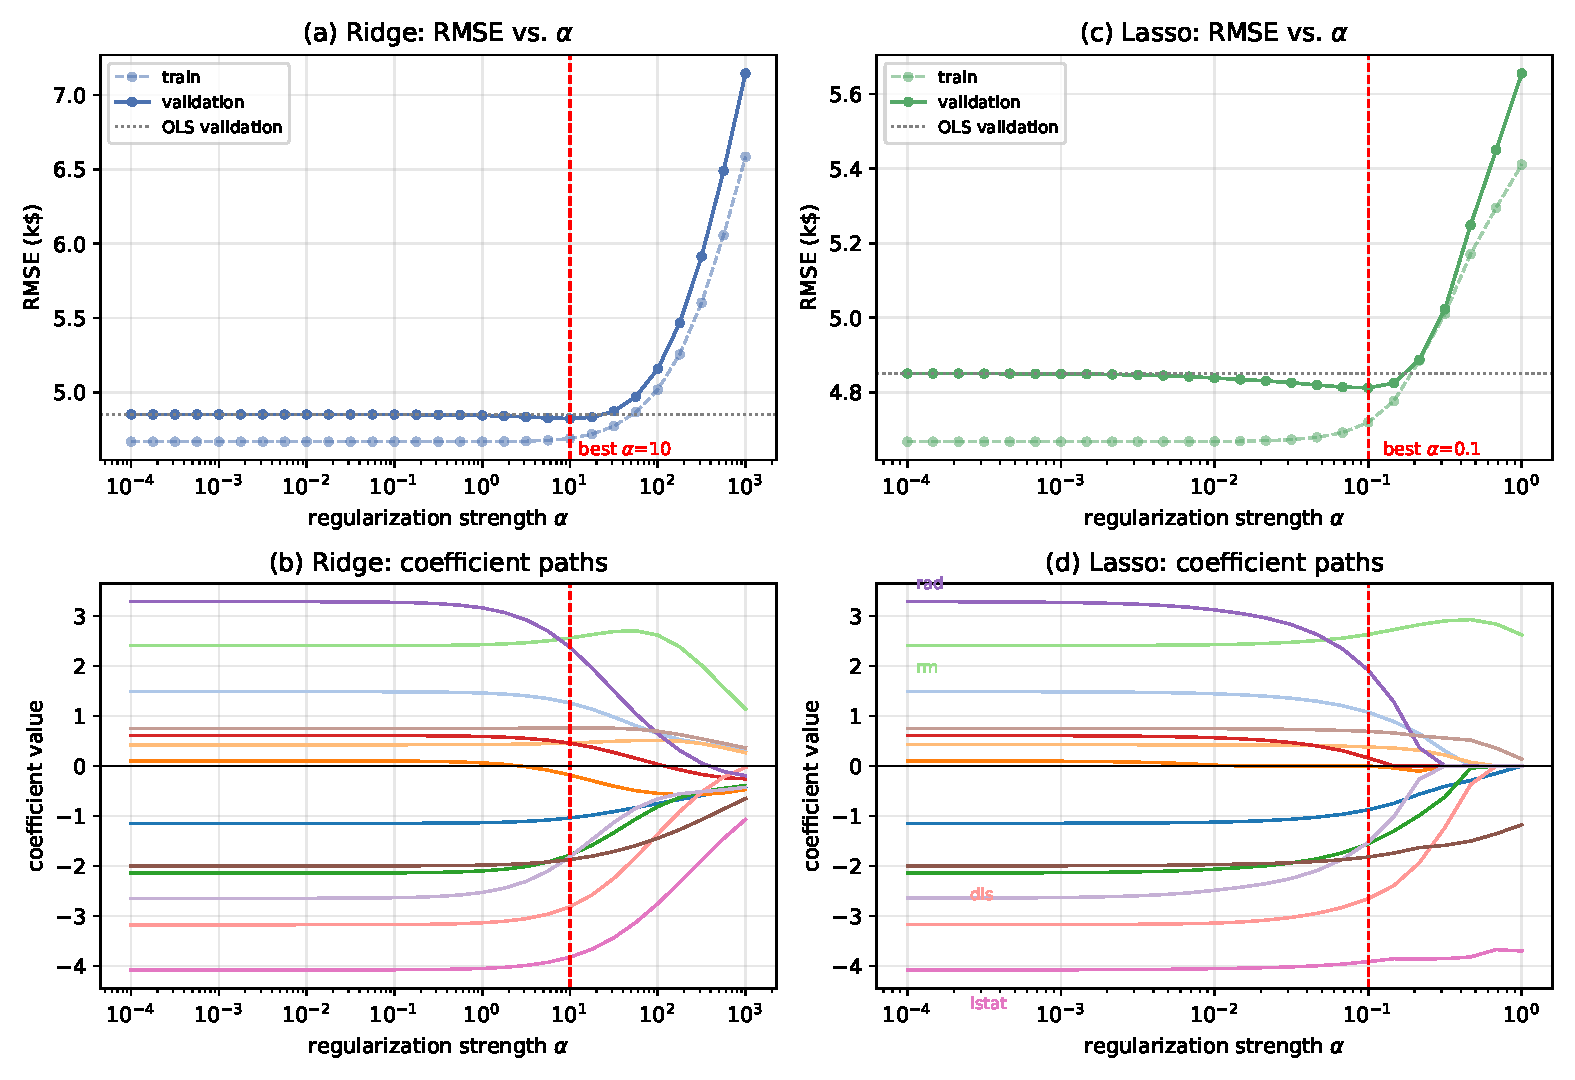
\includegraphics[width=\textwidth]{figures/boston_reg_paths.pdf}
  \caption{(a)(c) Ridge/Lasso 的训练与验证 RMSE 随 $\alpha$ 的变化（红色虚线为验证集最优 $\alpha$，灰色点线为 OLS 验证 RMSE）；(b)(d) 对应的系数路径。单条划分下最优 $\alpha$：Ridge 为 10，Lasso 为 0.1}
  \label{fig:paths}
\end{figure}

\begin{table}[H]
  \centering
  \caption{波士顿房价各模型结果对比（与作业2/3同一切分：train/val/test = 323/80/103；RMSE 与 MAE 单位：千美元）}
  \label{tab:main}
  \footnotesize
  \begin{tabular}{llcccc}
    \toprule
    方法 & 最优 $\alpha$ & RMSE$\downarrow$ & MAE$\downarrow$ & $R^2\uparrow$ & 非零系数数 \\
    \midrule
    OLS（baseline） & --- & 4.732 & 3.194 & 0.6824 & 13/13 \\
    Ridge & 10 & 4.694 & 3.091 & 0.6874 & 13/13 \\
    Lasso & 0.1 & \textbf{4.663} & \textbf{3.051} & \textbf{0.6917} & \textbf{12}/13 \\
    \midrule
    OLS + poly2 & --- & 3.876 & 2.672 & 0.7869 & 104/104 \\
    Ridge + poly2 & 17.8 & \textbf{3.245} & 2.342 & \textbf{0.8507} & 104/104 \\
    Lasso + poly2 & 0.1 & 3.337 & \textbf{2.333} & 0.8421 & \textbf{50}/104 \\
    \midrule
    Ridge（5 折交叉验证） & 每折内部重选参 & \multicolumn{2}{c}{$4.884\pm0.167$} & $0.7101\pm0.0393$ & --- \\
    Lasso（5 折交叉验证） & 每折内部重选参 & \multicolumn{2}{c}{$4.945\pm0.165$} & $0.7026\pm0.0402$ & --- \\
    \midrule
    MLPNN 13--64--32--1（作业2） & --- & 2.922 & 2.054 & 0.8789 & --- \\
    SVR-RBF（作业3） & --- & 3.070 & 2.157 & 0.8663 & --- \\
    \bottomrule
  \end{tabular}
\end{table}

\begin{figure}[H]
  \centering
  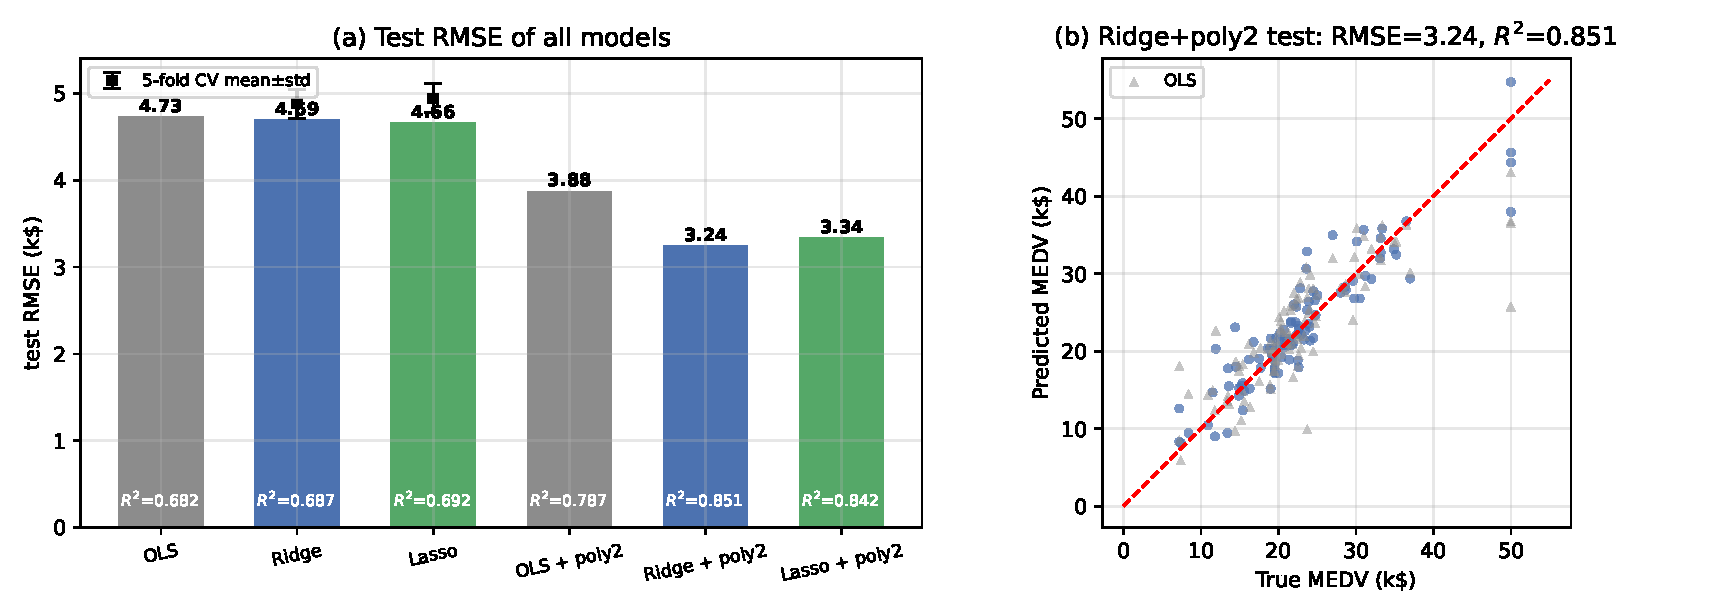
\includegraphics[width=\textwidth]{figures/boston_reg_comparison.pdf}
  \caption{(a) 各模型测试集 RMSE（方块与误差线为原始 13 维特征上 5 折交叉验证的均值$\pm$标准差）；(b) 最优正则化模型 Ridge+poly2 的测试集预测值--真实值散点（灰色三角为 OLS baseline）}
  \label{fig:cmp}
\end{figure}

\mlConclusion{1}
\begin{enumerate}
  \item 三种线性模型的测试集性能非常接近（Ridge/Lasso 仅比 OLS 略优 0.04--0.07 千美元），说明在仅 13 维、样本量 323 的情况下 OLS 的过拟合本就不严重，正则化的收益有限，但也没有损失；
  \item 由图~\ref{fig:paths}(a)(c) 可见典型的偏差--方差权衡：$\alpha$ 过大时训练与验证 RMSE 同时恶化（欠拟合）；对比 (b)(d) 两幅系数路径，Ridge 的系数随 $\alpha$ 平滑收缩、始终非零，而 Lasso 的系数被\textbf{逐个精确压到 0}（$\alpha=1$ 时仅剩 2 个非零），体现了 $\ell_1$ 惩罚的特征选择能力；
  \item 最优 Lasso（$\alpha=0.1$）将 indus 的系数压为 0（OLS 中其系数仅 0.10，为全特征最小），保留 12 个特征；三种模型系数排名一致，$|$coef$|$ 最大的始终是 lstat（负向，约 $-4.0$）、rad、dis、tax、rm（正向，约 $2.5$），与``低收入人口比例越低、房间数越多房价越高''的直觉相符；
  \item 单个系数看，Ridge 把 OLS 中量级冲突的 rad（3.29）与 tax（$-2.65$，二者高度共线：公路可达性好的地区税率往往也高）收缩为 2.37 与 $-1.82$，验证了 $\ell_2$ 惩罚缓解共线性的作用。
\end{enumerate}

\mlExperiment{5.2}{二阶多项式特征上的正则化对比}
为了考察正则化在高维特征下的价值，将特征做二阶多项式展开（13 维 $\to$ 104 维，含平方项与全部两两交叉项，展开后重新标准化），此时特征数已达训练样本数（323）的约三分之一，OLS 过拟合风险显著增加。同样以验证集 RMSE 选参，结果见表~\ref{tab:main} 与图~\ref{fig:cmp}。

\begin{figure}[H]
  \centering
  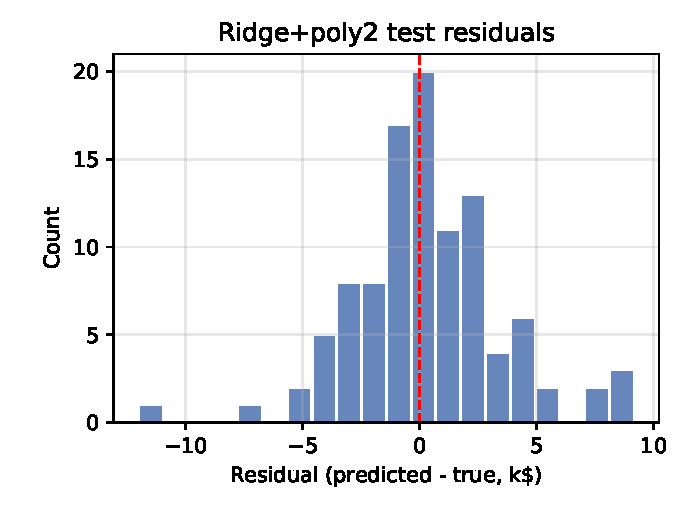
\includegraphics[width=0.5\textwidth]{figures/boston_reg_residuals.pdf}
  \caption{Ridge+poly2 的测试集残差直方图（预测值$-$真实值，千美元）}
  \label{fig:res}
\end{figure}

\mlConclusion{2}
\begin{enumerate}
  \item OLS+poly2 将测试 RMSE 从 4.73 降至 3.88（$R^2$ 0.787），说明房价中确实存在二阶非线性关系；但加入正则化后收益更大：Ridge+poly2 达 \textbf{RMSE 3.245、$R^2$ 0.851}，Lasso+poly2 达 RMSE 3.337，分别比同特征下的 OLS 提升 16\% 与 14\%，充分体现了正则化对高维模型的必要性；
  \item Lasso+poly2 在 104 个特征中仅保留 \textbf{50} 个非零系数即达到与 Ridge 相当的精度，模型更紧凑、可解释性更强；其选出的主要特征为 lstat、rm、lstat$^2$、tax$\times$lstat、tax$\times$ptratio、tax、nox$\times$rad 等——lstat 的平方项系数为正（$+2.79$）而一次项为负（$-4.25$），刻画了房价随 lstat 增大``先快后慢''下降的非线性饱和形态；
  \item 图~\ref{fig:cmp}(b) 与图~\ref{fig:res} 显示 Ridge+poly2 的预测点紧贴对角线、残差近似以 0 为中心对称分布，明显优于 OLS（灰色三角），但在 MEDV$=50$ 处仍系统性低估——该数据集的房价在 50 千美元处被人为截断，这一观测与作业2/3一致；
  \item 与作业2、作业3的非线性模型对比：Ridge+poly2（RMSE 3.245，$R^2$ 0.851）已接近 SVR-RBF（3.070，0.866）与 MLPNN（2.922，0.879）的水平，而训练只需解一次 $104\times104$ 的线性方程组（毫秒级），``特征工程 + 正则化线性模型''是该规模数据上极具性价比的方案。
\end{enumerate}

\mlExperiment{5.3}{5 折交叉验证}
为检验单次划分结论的稳健性，在全部 506 个样本上做 5 折交叉验证：每折内部独立进行标准化、划分验证集并重新在 $\alpha$ 网格上选参，模拟完整的训练+选参流程。

\mlConclusion{3}
5 折交叉验证下 Ridge 与 Lasso 的 RMSE 分别为 $4.884\pm0.167$ 与 $4.945\pm0.165$（$R^2$ 约 $0.70\pm0.04$），两者差异远小于折间标准差，再次确认两个模型在原始特征上性能相当；各折自动选出的 $\alpha$ 分布在 $10^{-4}$--32（Ridge）与 $2\times10^{-2}$--0.3（Lasso）之间，与单次划分选出的 10 / 0.1 相容，说明正则化强度的选择对数据划分不敏感、结论稳健。交叉验证 RMSE 高于单次划分的测试 RMSE，主要来自各折测试子集的样本构成差异（506 样本的小数据集上折间波动难免，作业2/3中也观察到了同样的现象）。

\section{总结}
本次作业设计并实现了以岭回归与 Lasso 为核心的波士顿房价预测回归系统。主要工作与结论：(1) 从零实现了岭回归的解析解与 Lasso 的坐标下降求解器（含软阈值更新与路径 warm start），与 scikit-learn 的实现差异在 $10^{-7}$ 以内；(2) 在原始 13 维特征上，Ridge（$\alpha=10$）与 Lasso（$\alpha=0.1$）相比 OLS 只有小幅提升（测试 RMSE 约 4.66--4.73 千美元），但 Lasso 能自动剔除无效特征（indus）、给出稀疏可解释的模型，系数路径实验清晰展示了 $\ell_1$ 的``精确置零''与 $\ell_2$ 的``平滑收缩''这两种正则化行为的本质差异；(3) 在二阶多项式特征（104 维）上，正则化的价值充分体现：Ridge+poly2 取得 RMSE 3.245、$R^2$ 0.851 的全系统最好成绩，比同特征 OLS 提升 16\%，接近作业2/3中 MLPNN 与 SVR-RBF 的水平而计算开销低数个量级，Lasso+poly2 则以一半的非零系数达到了相当的精度；(4) 5 折交叉验证确认超参数选择与模型对比结论稳健。后续可尝试 ElasticNet（$\ell_1+\ell_2$ 组合）在共线性强的高维特征上兼顾稀疏性与分组选择，或用核岭回归直接对比 RBF 核方法。

\end{document}
